\section{Thiết lập thực nghiệm}

\subsection{Khu vực nghiên cứu}

Theo Nghị quyết số 1278/NQ-UBTVQH15 ngày 24/10/2024 của Ủy ban Thường vụ Quốc hội, kể từ ngày 01/07/2025, tỉnh Cà Mau và tỉnh Bạc Liêu được sáp nhập thành tỉnh Cà Mau mới với tổng diện tích tự nhiên 7.942,38 km² và dân số khoảng 2,6 triệu người. Đồ án này nghiên cứu trên phạm vi rừng của tỉnh Cà Mau mới, bao gồm cả vùng rừng thuộc địa bàn Bạc Liêu cũ.

Tỉnh Cà Mau mới nằm ở cực Nam Tổ Quốc, sở hữu hệ sinh thái rừng đa dạng bao gồm cả rừng ngập mặn ven biển và rừng tràm nội địa. Theo số liệu trước khi sáp nhập, tỉnh Cà Mau cũ có diện tích rừng khoảng 94.319 ha và tỉnh Bạc Liêu có khoảng 5.730 ha rừng, tổng cộng khoảng 100.000 ha rừng trên toàn tỉnh Cà Mau mới \citevi{snnptntcamau2021}. Trong đó, rừng ngập mặn Cà Mau chiếm khoảng 20\% diện tích rừng ngập mặn của Việt Nam. Hệ thống rừng tại Cà Mau đóng vai trò then chốt trong việc phòng hộ ven biển (chắn sóng, chống xâm thực và bảo vệ bờ biển), bảo tồn đa dạng sinh học vì là môi trường sống cho nhiều loài động thực vật quý hiếm, cung cấp nguồn sinh kế thông qua các hoạt động thủy sản và du lịch sinh thái, và góp phần giảm nhẹ biến đổi khí hậu nhờ khả năng lưu giữ carbon cao, gấp khoảng 3–5 lần so với rừng nhiệt đới trên cạn \citeen{donato2011,alongi2014}.

Tuy nhiên, rừng Cà Mau đang phải đối mặt với nhiều thách thức. Trước hết là áp lực chuyển đổi sang nuôi tôm do kinh tế, khiến nhiều khu vực rừng bị chuyển đổi thành ao nuôi. Ngoài ra, hiện tượng xâm nhập mặn gia tăng do biến đổi khí hậu làm giảm sức khỏe rừng; đồng thời xói mòn bờ biển cũng làm suy giảm diện tích rừng ven biển; và tình trạng thiếu nước ngọt ảnh hưởng tới khả năng tái sinh tự nhiên của rừng. Giai đoạn 2011--2023, sạt lở vùng ven biển đã làm mất hơn 6.200 ha đất và rừng phòng hộ \citevi{nongnghiepmoitruong2024}.

Để hiểu rõ bối cảnh không gian và đa dạng lớp phủ bề mặt tại khu vực nghiên cứu, Hình~\ref{fig:camau_lulc} trình bày bản đồ phân loại lớp phủ/sử dụng đất (LULC) tỉnh Cà Mau. Phân loại LULC cung cấp thông tin nền tảng về các loại hình sử dụng đất khác nhau trên địa bàn, từ đó giúp xác định ranh giới giữa vùng rừng và phi rừng, cũng như các vùng có nguy cơ chuyển đổi cao \citeen{gong2013}. Bản đồ này được xây dựng từ dữ liệu viễn thám từ Esri phản ánh hiện trạng sử dụng đất phức tạp tại tỉnh Cà Mau, nơi mà sự tương tác giữa các hệ sinh thái tự nhiên (rừng ngập mặn, đất ngập nước) và các hoạt động kinh tế-xã hội (nuôi trồng thủy sản, nông nghiệp) diễn ra liên tục \citeen{renaud2015}.

Phân tích bản đồ cho thấy sự phân bố không đồng nhất của các loại hình lớp phủ, với rừng ngập mặn tập trung chủ yếu dọc bờ biển phía Tây và Nam, trong khi các vùng nuôi trồng thủy sản và nông nghiệp lúa nước chiếm ưu thế ở khu vực trung tâm và phía Đông. Mô hình phân bố này phản ánh lịch sử khai thác và quản lý tài nguyên tại Cà Mau, đồng thời làm nổi bật sự cần thiết phải có công cụ giám sát biến động rừng hiệu quả để hỗ trợ các quyết định quản lý bền vững \citeen{kuenzer2011}.

Đồ án tập trung vào toàn bộ vùng quy hoạch lâm nghiệp của tỉnh Cà Mau mới. Dữ liệu ranh giới quy hoạch lâm nghiệp được cung cấp bởi Công ty TNHH Tư vấn và Phát triển Đồng Xanh — đối tác của Chi cục Kiểm lâm tỉnh Cà Mau.

Tổng diện tích ranh giới quy hoạch là 170.178,82 ha (tương đương 1.701,79 km²), bao gồm 666 polygon trong file shapefile ranh giới. Diện tích thực tế được phân loại là 162.468,50 ha (khoảng 95,5\% diện tích ranh giới); phần còn lại (~7.710 ha, chiếm 4,5\%) bị loại do mây che phủ hoặc dữ liệu không hợp lệ (nodata) trong quá trình xử lý ảnh vệ tinh. Kích thước raster là 12.547 × 10.917 điểm ảnh (ở độ phân giải 10m), sử dụng hệ quy chiếu EPSG:32648 (WGS 84 / UTM Zone 48N).

\subsection{Dữ liệu thực địa tại Cà Mau}

Dữ liệu thực địa được Công ty TNHH Tư vấn và Phát triển Đồng Xanh (GFD) thu thập trong khuôn khổ thực hiện đề tài ``Ứng dụng công nghệ viễn thám, ảnh vệ tinh để quản lý, giám sát tài nguyên rừng và sạt lở ven biển trên địa bàn tỉnh Cà Mau'' \citevi{gfd2025} và được cung cấp cho nghiên cứu này. Quy trình thu thập gồm ba giai đoạn. Giai đoạn đầu tiên là khảo sát thực địa bằng thiết bị bay không người lái (drone) để ghi nhận hình ảnh và xác định trạng thái rừng. Giai đoạn thứ hai là số hóa các điểm dữ liệu thực địa trên phần mềm QGIS, đối chiếu với ảnh vệ tinh Sentinel-2. Giai đoạn cuối cùng là kiểm tra chéo và loại bỏ các điểm không rõ ràng hoặc nằm trong vùng mây che phủ. Dữ liệu cuối cùng được xuất dưới dạng file CSV với cấu trúc gồm 4 trường: \textit{id}, \textit{label}, \textit{x} và \textit{y} (tọa độ theo hệ quy chiếu EPSG:32648).

\begin{table}[H]
\centering
\caption{Thống kê dữ liệu thực địa theo lớp biến động}
\label{tab:ground_truth}
\begin{tabular}{|c|l|c|c|l|}
\hline
\textbf{Lớp} & \textbf{Tên} & \textbf{Số điểm} & \textbf{Tỷ lệ} & \textbf{Mô tả} \\
\hline
0 & Rừng ổn định & 656 & 24,9\% & Có rừng ở cả 2 kỳ \\
\hline
1 & Mất rừng & 650 & 24,7\% & Có rừng $\rightarrow$ không có rừng \\
\hline
2 & Phi rừng & 664 & 25,3\% & Không có rừng ở cả 2 kỳ \\
\hline
3 & Phục hồi rừng & 660 & 25,1\% & Không có $\rightarrow$ có rừng \\
\hline
\textbf{Tổng} & & \textbf{2.630} & \textbf{100\%} & Phân bố cân bằng \\
\hline
\end{tabular}
\end{table}

Phân bố không gian của các điểm dữ liệu thực địa được minh họa trong Hình~\ref{fig:ground_truth_map}. Các điểm mẫu được thu thập phân tán trên toàn bộ khu vực nghiên cứu, đảm bảo tính đại diện về mặt không gian cho các loại hình biến động rừng khác nhau.

\begin{figure}[H]
\centering
\includegraphics[width=0.9\textwidth]{chapter3/samples.png}
\caption{Bản đồ phân bố không gian các điểm dữ liệu thực địa trên khu vực nghiên cứu tỉnh Cà Mau}
\label{fig:ground_truth_map}
\end{figure}

Mỗi điểm ảnh trong bộ dữ liệu được biểu diễn bởi 27 đặc trưng: 9 đặc trưng tại thời điểm $T_1$, 9 đặc trưng tại thời điểm $T_2$, và 9 đặc trưng delta ($\Delta = T_2 - T_1$). Mô hình CNN sử dụng toàn bộ 27 đặc trưng này làm đầu vào để tận dụng tối đa thông tin từ cả hai thời điểm quan sát. Tuy nhiên, để phân tích trực quan khả năng phân biệt của dữ liệu, nghiên cứu lựa chọn minh họa 9 đặc trưng delta thông qua (Hình~\ref{fig:pairplot_delta}). Việc lựa chọn này xuất phát từ hai lý do chính. Thứ nhất, biểu đồ Phân bố với 27 đặc trưng sẽ tạo ra ma trận $27 \times 27 = 729$ ô, quá lớn để quan sát và phân tích hiệu quả. Thứ hai, đặc trưng delta trực tiếp biểu diễn sự thay đổi giữa hai thời điểm, do đó phù hợp nhất để đánh giá khả năng phân tách các lớp biến động rừng.

\begin{figure}[H]
\centering
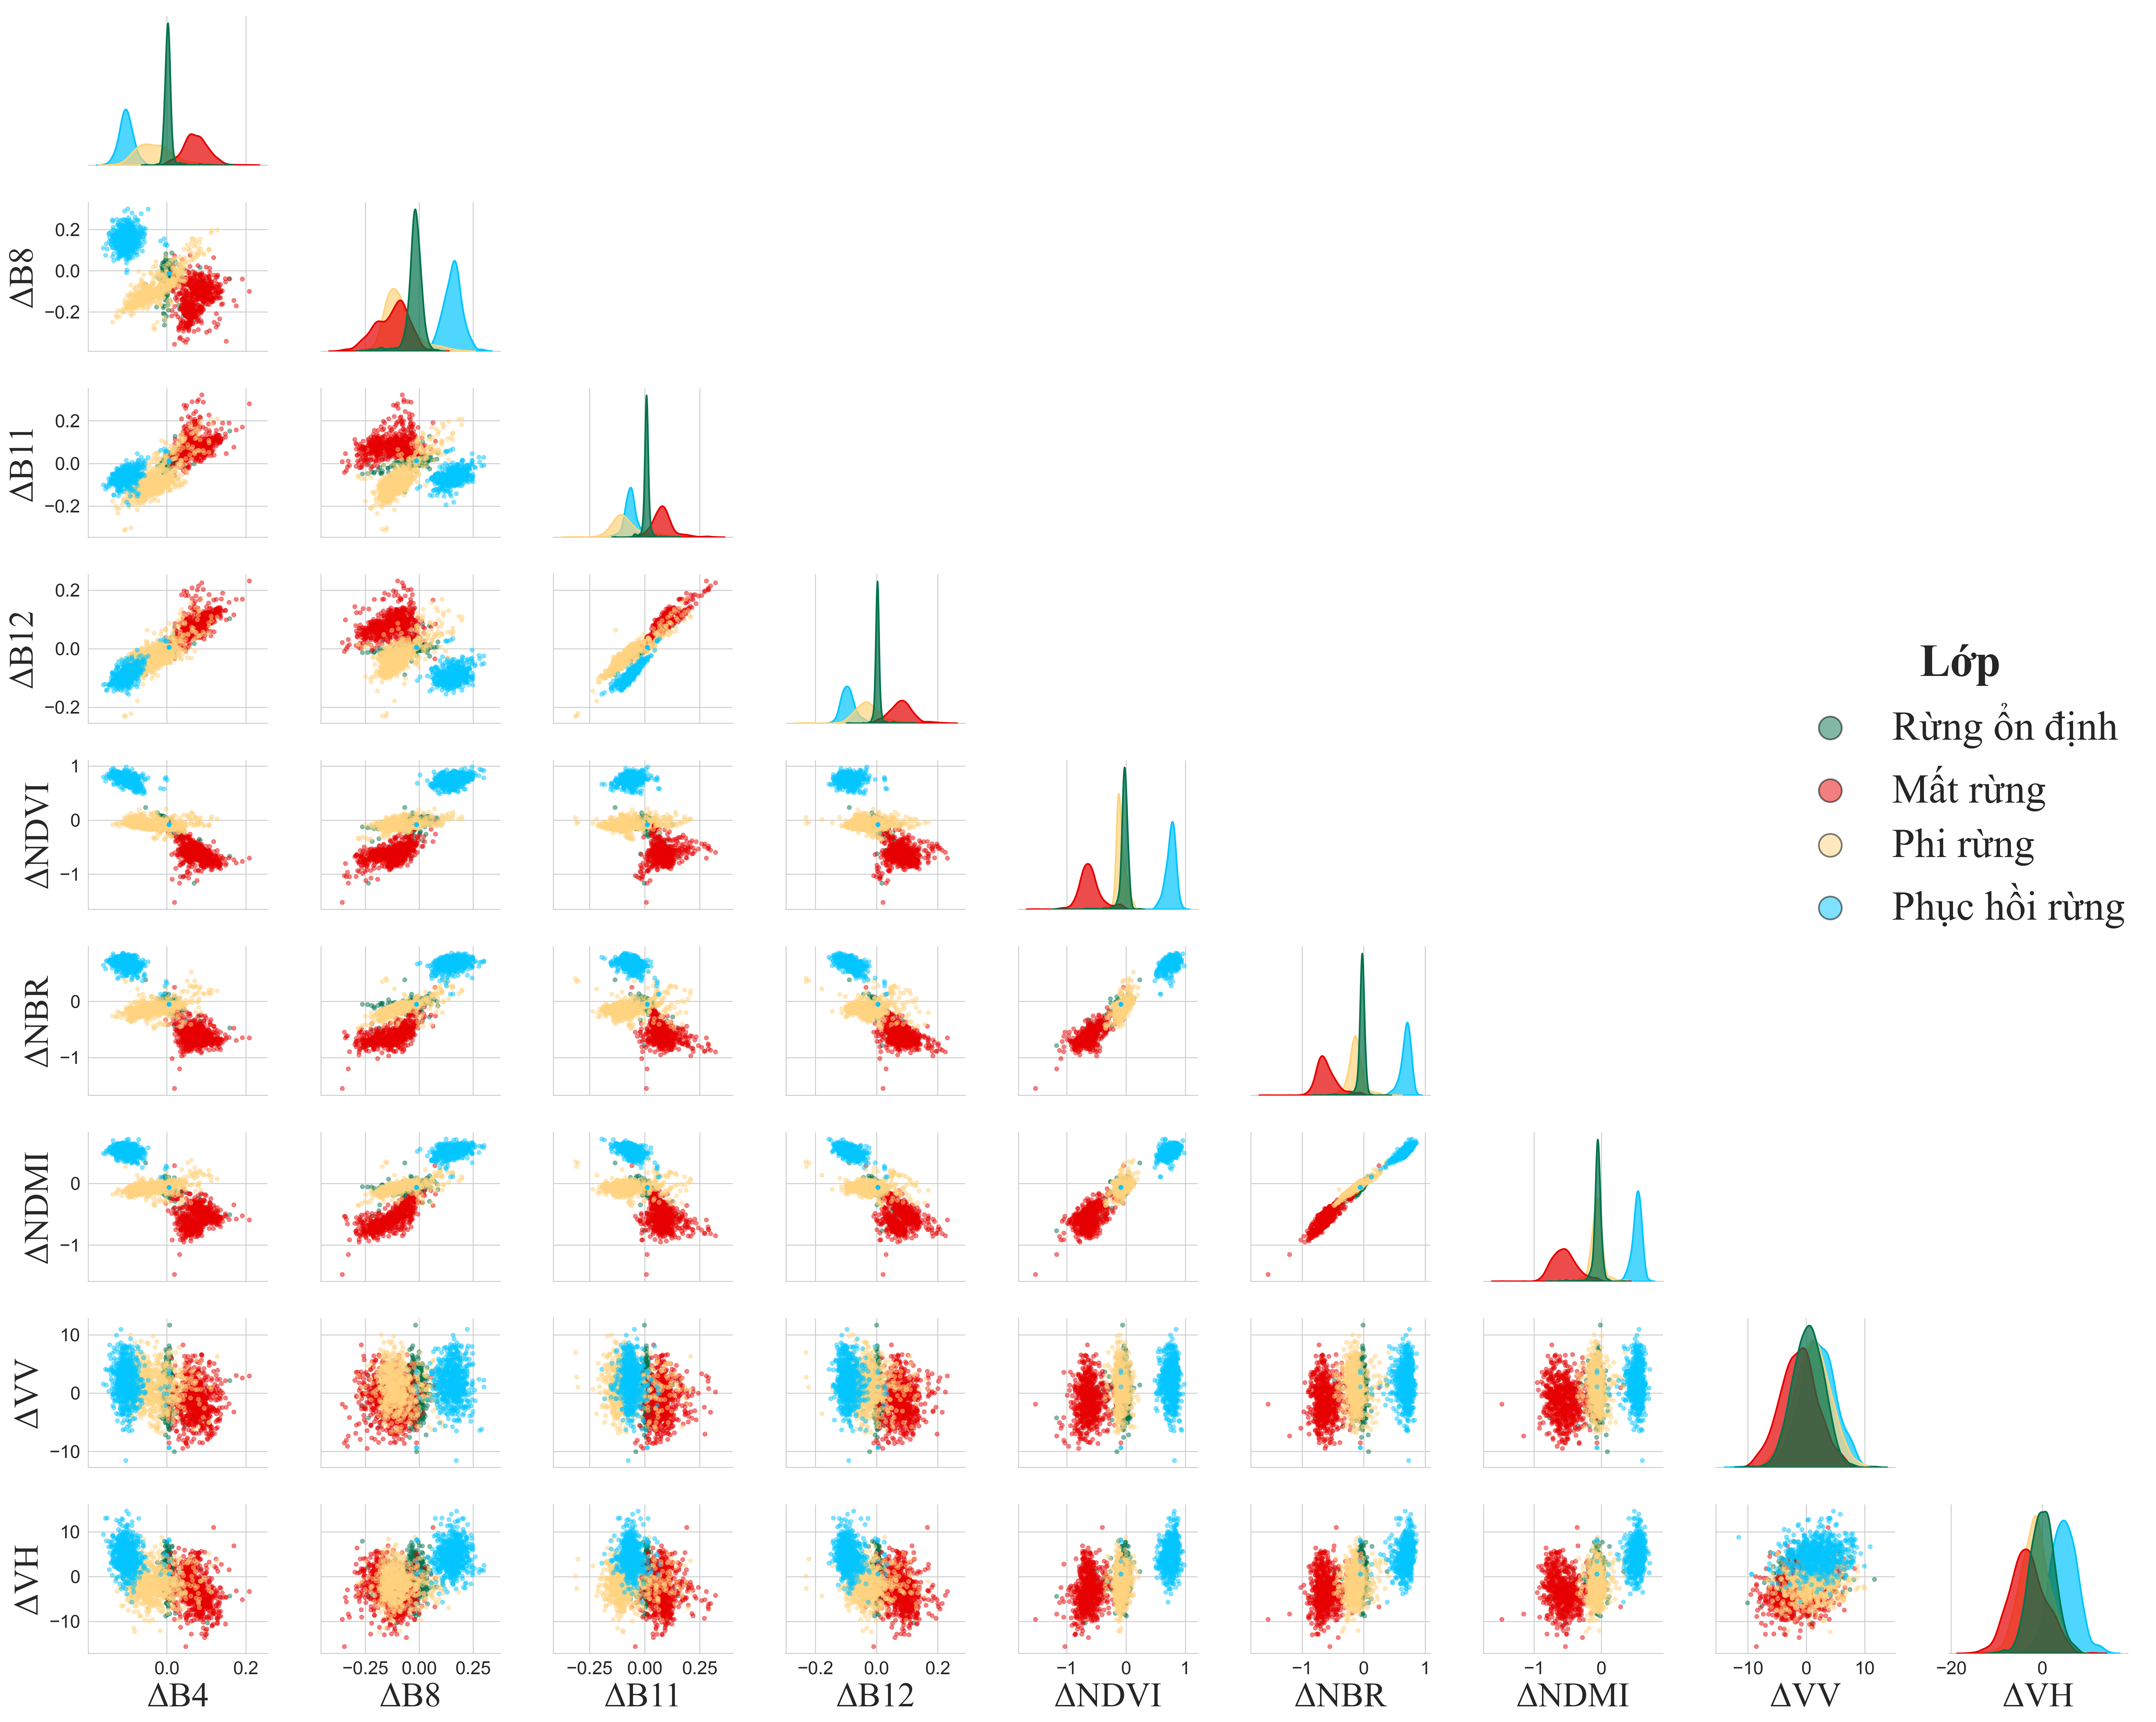
\includegraphics[width=0.95\textwidth]{img/chapter3/pairplot_delta_features.png}
\caption{Phân bố các đặc trưng delta theo lớp biến động rừng}
\label{fig:pairplot_delta}
\end{figure}

Biểu đồ trình bày mối quan hệ giữa 9 đặc trưng delta bao gồm các band quang phổ Sentinel-2 ($\Delta$B4, $\Delta$B8, $\Delta$B11, $\Delta$B12), các chỉ số thực vật ($\Delta$NDVI, $\Delta$NBR, $\Delta$NDMI) và các kênh ra-đa Sentinel-1 ($\Delta$VV, $\Delta$VH). Trên đường chéo chính, biểu đồ thể hiện phân bố của từng đặc trưng theo bốn lớp biến động; các ô còn lại hiển thị biểu đồ tán xạ giữa các cặp đặc trưng.

Phân tích phân bố trên đường chéo cho thấy các chỉ số thực vật delta thể hiện khả năng phân biệt vượt trội giữa các lớp biến động. Cụ thể, lớp Rừng ổn định và Phi rừng có phân bố tập trung quanh giá trị 0, phản ánh sự ổn định về lớp phủ thực vật qua hai thời điểm quan sát. Ngược lại, lớp Mất rừng thể hiện phân bố lệch về phía âm do sự suy giảm các chỉ số thực vật khi rừng bị chuyển đổi, trong khi lớp Phục hồi rừng có phân bố lệch về phía dương tương ứng với sự gia tăng sinh khối thực vật. Sự phân tách rõ ràng này khẳng định vai trò then chốt của $\Delta$NDVI, $\Delta$NBR và $\Delta$NDMI trong việc nhận diện biến động rừng.

Đối với các band quang phổ gốc, mức độ chồng chéo giữa các lớp cao hơn so với các chỉ số thực vật, tuy nhiên $\Delta$B8 (kênh cận hồng ngoại) vẫn cho thấy khả năng phân biệt tương đối tốt giữa lớp Mất rừng và Phục hồi rừng. Các đặc trưng ra-đa $\Delta$VV và $\Delta$VH có phân bố chồng chéo đáng kể giữa bốn lớp, cho thấy khả năng phân biệt độc lập hạn chế hơn so với dữ liệu quang học. Tuy nhiên, việc tích hợp dữ liệu ra-đa vẫn mang lại giá trị bổ sung, đặc biệt trong điều kiện mây che phủ thường xuyên tại khu vực nghiên cứu.

Phân tích các biểu đồ tán xạ cho thấy mối tương quan dương mạnh giữa ba chỉ số thực vật ($\Delta$NDVI, $\Delta$NBR, $\Delta$NDMI), thể hiện qua sự phân bố các điểm dữ liệu gần đường chéo. Tương tự, $\Delta$B11 và $\Delta$B12 có tương quan cao do cùng thuộc dải sóng ngắn hồng ngoại (SWIR). Trên không gian đặc trưng hai chiều của các chỉ số thực vật, lớp Mất rừng và Phục hồi rừng phân bố ở hai vùng đối lập nhau, trong khi lớp Rừng ổn định và Phi rừng tập trung quanh gốc tọa độ. Đặc điểm phân bố này tạo điều kiện thuận lợi cho mô hình CNN trong việc học các ranh giới quyết định phân tách bốn lớp biến động.

\subsection{Cấu hình phần cứng và phần mềm}

Môi trường thí nghiệm sử dụng phần cứng với CPU Intel Xeon E-2334 (4 nhân, 8 luồng), GPU NVIDIA GeForce RTX 4080 (16GB VRAM), bộ nhớ RAM 64GB và bộ nhớ lưu trữ 1TB SSD. Về phần mềm, hệ điều hành được sử dụng là Windows 10 Pro, môi trường Python 3.11 cùng PyTorch 2.5 có hỗ trợ CUDA 12.1 để huấn luyện mô hình, rasterio 1.4 (GDAL 3.6) cho xử lý dữ liệu không gian và các thư viện khoa học dữ liệu như NumPy, scikit-learn và pandas.

PyTorch được lựa chọn làm framework học sâu chính cho nghiên cứu này vì một số lý do. Thứ nhất, PyTorch sử dụng cơ chế đồ thị tính toán động (dynamic computational graph), cho phép xây dựng và sửa đổi kiến trúc mô hình một cách linh hoạt trong quá trình thử nghiệm. Thứ hai, cú pháp của PyTorch gần gũi với Python thuần túy, giúp việc triển khai và gỡ lỗi mô hình trở nên trực quan hơn. Thứ ba, PyTorch được hỗ trợ bởi cộng đồng nghiên cứu rộng lớn với nhiều mô hình tiền huấn luyện và thư viện mở rộng như torchvision, torchaudio. Cuối cùng, khả năng tích hợp tốt với CUDA cho phép tận dụng hiệu quả GPU trong quá trình huấn luyện và suy luận.

\subsection{Phân chia dữ liệu}

Bộ dữ liệu thực địa gồm 2.630 điểm, trong đó phân bố lớp gần như cân bằng: Lớp 0 (Rừng ổn định) 656 điểm (24,94\%), Lớp 1 (Mất rừng) 650 điểm (24,71\%), Lớp 2 (Phi rừng) 664 điểm (25,25\%) và Lớp 3 (Phục hồi rừng) 660 điểm (25,10\%).

\begin{table}[H]
\centering
\caption{Phân bố dữ liệu theo tập huấn luyện và kiểm tra}
\label{tab:data_split_info}
\begin{tabular}{|l|c|c|}
\hline
\textbf{Tập dữ liệu} & \textbf{Số mẫu} & \textbf{Tỷ lệ} \\
\hline
Huấn luyện + Kiểm định (5-Fold CV) & 2.104 & 80\% \\
\hline
Kiểm tra (cố định) & 526 & 20\% \\
\hline
\textbf{Tổng} & \textbf{2.630} & \textbf{100\%} \\
\hline
\end{tabular}
\end{table}

Việc chia tập dữ liệu được thực hiện như sau: 80\% dữ liệu (2.104 patches) được dành cho Huấn luyện + Kiểm định để thực hiện Kiểm định chéo 5 phần, còn 20\% dữ liệu (526 patches) được giữ lại làm tập dữ liệu kiểm tra cố định.

Kết quả trên hoàn thành mục tiêu thứ nhất, xây dựng bộ dữ liệu huấn luyện gồm 2.630 điểm mẫu với 27 đặc trưng từ ảnh vệ tinh Sentinel-1 và Sentinel-2 đa thời gian, bao gồm các kênh phổ, chỉ số thực vật và tán xạ ngược cho khu vực quy hoạch lâm nghiệp tỉnh Cà Mau.
